\scanpage{76}
De plus, $J_{A/k}$ est \uline{projectif} \uline{relativement aux suites exactes loc. triviales}.
\inserted{i.e. son $\uline{\operatorname{Ext}^1}$ \unsure{avec} \uline{un \unsure{grpe|gpe} \unsure{lin.} connexe est $0$}.}

\noindent c) Si $\dim A\geq2$, alors $J_{A/k}$ est \uline{connexe}, \uline{unipotent} (i.e. plus de partie abélienne ni multiplicative) et de plus \uline{projectif} (car le foncteur \unsure{qu'elle|qu'il} représente est exact\inserted{)}\deleted{, comme pour $\dim A=1$)}
\figure{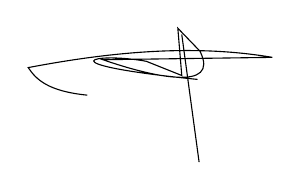
\begin{tikzpicture}[x=1cm,y=1cm]
\draw (0,0) .. controls (-.5,.05) and (-.65,.2) .. (-.75,.35) .. controls (.3,.55) and (1.35,.65) .. (2.35,.48) --(.2,.45) .. controls (.8,.24) and (1.7,.03) .. (1.43,.56) --(1.15,.85) --(1.2,.25) --(.75,.43) .. controls (.1,.55) and (-.6,.4) .. (1.4,.2);
\draw (1.2,.77)--(1.42,-.85);
\end{tikzpicture}}
% archive sheet number: 75
